\section{Theory and experimental setup}

\subsection{Fluorescence Photophysics} \label{sec:fluorescence_photophysics}
Fluorescence is a property of some substances describing their ability to capture photons and re-emit a photon of lower energy after a small duration. This phenomenon can be explained by the fluorescent particle transitioning from its ground state to an excited state, after which it relaxes to a lower energy state. The decay back to the ground state then causes the emission of a photon of a higher wavelength (and thus lower energy) than the excitation photon due to energy lost in the transition to a lower energy excited state. It is also possible for the fluorescent particle to decay without emitting a photon. These transitions usually happen on time scales of the order of $10^{-9}$ seconds \cite{douglass_notice_2023}.

Commonly, fluorophores have multiple energy levels to which the excited state can decay to, as depicted in \autoref{fig:energy_level_fluorophore}. For them to function properly for microscopy, the fluorophores have to be mixed in a buffer that provides reagents for the fluorophores to return to their ground state. After being excited by an incident photon, there is a small probability that the fluorophore decays to a lower excited state ($^3\textrm F$ in the figure). In this state, it can react with the compounds in the buffer to either return to the ground state or reach a third excited state, the radical anion state. This state is quite unreactive and therefore has a much longer lifetime than the other states.
\begin{figure}[htbp]
    \centering
    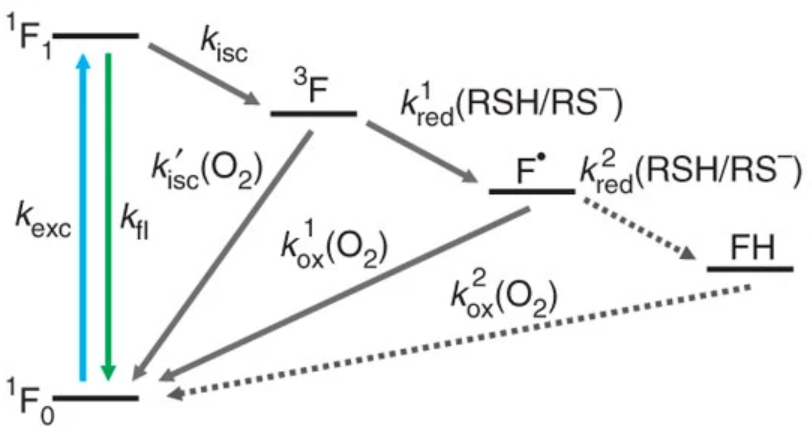
\includegraphics[width=0.7\textwidth]{figures/alexafluor-jablonski-diagram.png}
    \caption{Energy level diagram of fluorophores from the Alexafluor and ATTO families \cite{vandelinde-natureprotocols-2011}}
    \label{fig:energy_level_fluorophore}
\end{figure}

In the radical anion state, the fluorophore can be considered \enquote{disabled} or \textsc{off}, as it does not fluoresce. Fluorophores that can fluoresce are referred to as being \textsc{on}. Some fluorophores may get stuck in an \textsc{off} state, a \textsc{bleached} state. \emph{Photoswitching} is a technique that aims to control the number of fluorophores in the \textsc{on} and \textsc{off} state by modulating the compounds in the buffer, the light intensity, and through the use of different illumination wavelengths on the sample. 
% This technique is the basis for STORM.


\subsection{The Point Spread Function} \label{sec:PSF}
All optical microscopes have a limited resolution for how small a point-like light source can appear. The shape of the point measured in through the microscope is described by the point spread function, or PSF, which caracterises the performance of a particular microscope. The light intensity $I(x, y)$ of point-like light sources as measured by the microscope can then be described as a convolution between the density of emitters $O(x, y)$ and the PSF:
\begin{equation}
    I(x, y) = \operatorname{PSF}(x, y) \star O(x, y)
\end{equation}
Under the assumption that the PSF is only influenced by the diffraction of light, its form can be found to be an Airy Disk, which is mathematically described by
\begin{equation}
    I(X) = I_0 \left[ \frac{2 J_1(X)}{X} \right]^{2}, \quad X = \frac{2\pi r \textrm{NA}}{\lambda}
\end{equation}
where $r=\sqrt{x^2+y^2}$ is the radial coordinate, NA is the numerical aperture of the optical system, $\lambda$ is the wavelength of the light, and $J_1$ is the first order Bessel function of the first kind. The size or width of the PSF can then be defined by the first zero of the Airy disk, located at $\Delta X \approx 3.8317$, or $\Delta r \approx 0.61 \lambda / \textrm{NA}$.

\subsection{Single Molecule Localization Microscopy} \label{sec:SMLM}
In most cases, the smallest object an optical microscope can observe has a size of about half of the wavelength of light. However, a fluorescent molecule as observed through the microscope is located in the middle of the image it produces, that is, its PSF. By fitting the PSF to the image of a single molecule, its position can be estimated with a precision on the order of 10 nm for visible light \cite{douglass_notice_2023}, which is much more precise than what the wavelength of visible light would allow. This technique is called single molecule localization microscopy, or SMLM. Multiple fitting techniques exist, each with their advantages and disadvantages. In this report, a two-dimensional Gaussian curve of the following form will be used as an approximation of the Airy disk intensity function to the image, as it is more efficient \mbox{computationally \cite{douglass_notice_2023}}:
\begin{equation}
    f(x, y) = a \exp \left[ \frac{(x-\mu_x)^2 + (y-\mu_y)^2}{2 \sigma^2} \right] + b
\end{equation}
where $\mu_x$ and $\mu_y$ give the position of the molecule and $\sigma$ is the standard deviation, which can be related to the wavelength and numerical aperture through \cite{zhang-appliedoptics-2007}
\begin{equation}
    \sigma \approx 0.21 \frac{\lambda}{\textrm{NA}}
    \label{eq:PSF_width_gaussian}
\end{equation}


\subsection{STORM} \label{sec:STORM}
The gaussian fitting allows to locate an isolated molecule, but as a consequence of the uncertainty associated, two fluorescent molecules whose images overlap are impossible to localize.
The localization of dense distributions of emitters, such as fluorophores attached to cellular structures, must therefore be carried out with techniques more complex than the capture of a single image.
One such technique based on photoswitching is stochastic optical reconstruction microscopy (STORM).
It relies on the principle that we can localize all the fluorophores in an image by keeping only part of them in the \textsc{on} state  at a time.
By then capturing a large number of images, each with a stochastically determined subset of fluorophores switched on, and by localizing the molecules in each image, a list of all resolved emitter positions can be obtained, from which a super-resolved image is rendered.

For this technique to be effective, the density of molecules being read out
(that is, in an emissive state) at the same time must stay low
enough for the distance between emitting molecules to be large
compared to the diffraction limit, so that individual fluorophores
can be spatially \mbox{resolved \cite{furstenberg_single-molecule_2013}}.
This is accomplished by finetuning the parameters involved in photoswitching, as mentioned in \autoref{sec:fluorescence_photophysics}.


\subsection{Image reconstruction} \label{sec:imaging}
Once the positions of all the single fluorescence emitters have been determined, there are many possible ways to reconstruct an image.
The simplest would be to draw a point of fixed intensity in every localization position, or to draw a two-dimensional histogram by defining a pixel grid and assigning to each pixel an intensity proportional to the number of localised molecules contained.
These two approaches, however, often do not form a good representation of the imaged structure, both for reasons of accuracy and aesthetical clarity.
In this experiment, the approach taken was the one described in detail in \cite{martens_raw_2022}:
the positions of the molecules were plotted together with their uncertainty, by drawing in each position a normalised Gaussian intensity distribution.
In this way, the images appear less dotty and connected structures and increased spot densities are better recognisable.


\subsection{Epifluorescence Microscopes} \label{sec:epifluorescence_microscopes}
A common architecture for fluorescence microscopes is that of an upright epifluorescence microscope, pictured in \autoref{fig:epifluorescence_microscope}.
%
\begin{figure}[htbp]  
    \centering
    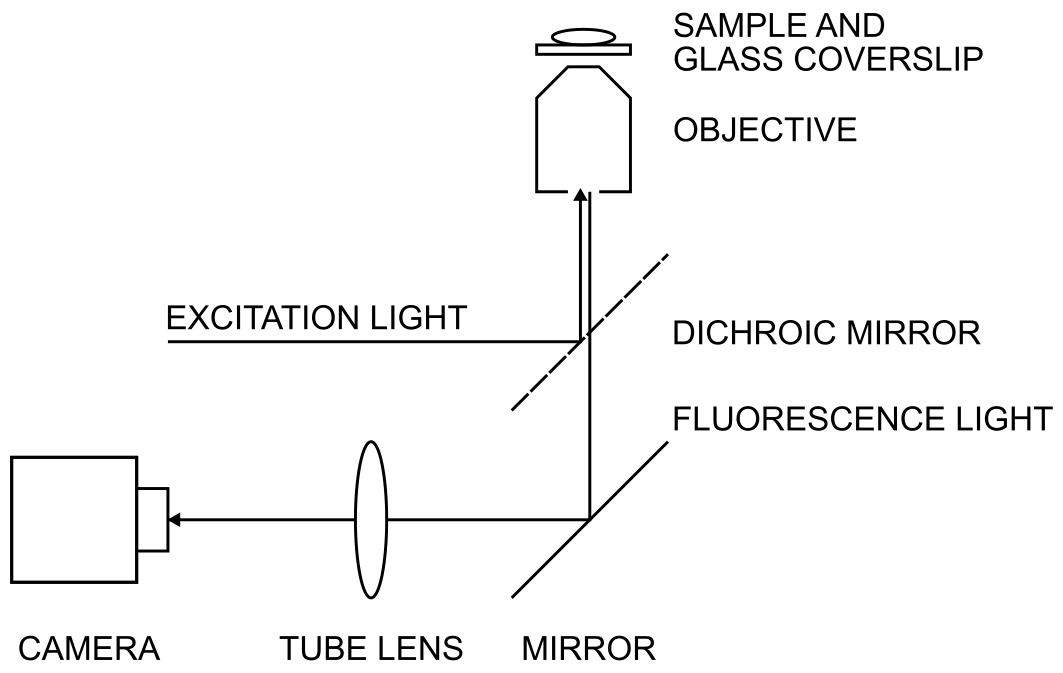
\includegraphics[width=8cm]{figures/epifluorescence-microscope.png}
    \caption{Epifluorescence microscope \cite{douglass_notice_2023}}
    \label{fig:epifluorescence_microscope}
\end{figure}
%
Light emitted from a source such as a laser or a high-intensity LED enters the microscope and is reflected into the objective lens by a dichroic mirror, capable of reflecting some wavelengths of light and transmitting others.
The excitation light is then focused by the objective lens onto the studied sample, where it excites the fluorescent molecules present.
The fluorescent light emitted by the molecules is collimated by the same objective lens and passes again through the dichroic mirror, which acts as a beam splitter, separating the excitation and emission light paths \cite{sachl_introduction_2022}.
Finally, a second lens, known as tube lens, focuses the parallel rays coming from the objective lens and forms the image of the sample on the camera or eyepiece.
This setup using two lenses is called an infinity-corrected system and allows to add or replace optical elements, such as filters or additional beamsplitters, in the \emph{infinity space} between the two lenses  without modifying the wavefront of the light, and thus keeping the same focus and magnification.

This mode of observation, where the excitation light is delivered to the specimen by the same objective lens which is used for collecting the fluorescence, is known as epi-illumination.
It is particularly useful to solve the problem of the excitation light dominating the weaker fluorescence signal, as most of the excitation light propagates away from the objective after leaving the sample \cite{douglass_notice_2023}.


\subsection{A bit of biology} \label{sec:biology}
In this report the following structures from eukaryotic cells, i.e. cells possessing a membrane-bound nucleus, were studied:
\begin{itemize}
    \item Microtubules: hollow, cylindrical polymers of tubulin proteins which measure 25 nm
    in diameter and vary in length from a fraction of a micrometer to hundreds of \mbox{micrometers \cite{lodish_molecular_2004}.}
    They are one of the components forming the cytoskeleton, the network of filaments that extends from the nucleus to the membrane and gives the cell its shape \cite{douglass_notice_2023}.
    \item Mitochondria: energy-transforming and signaling organelles that constitute part of the cell information processing system \cite{picard_mitochondrial_2022}. They are diverse in shapes and size, with a usual cross section between $0.75$ and $3$ \unit{\micro\meter\squared} \cite{wiemerslage_quantification_2016}.
    \item Clathrin: a protein involved in the formation of vesicles, on the cytoplasmatic side of the cell. 
    Clathrin-coated pits allow for molecules from the extracellular environment to be transported into the cell \cite{douglass_notice_2023}.
\end{itemize}


\subsection{Experimental setup} \label{sec:experimental_setup}
This experiment was carried out using an Abbelight SAFe 180 Single Molecule Localization Microscope, coupled to a laser engine and a Hamamatsu digital CMOS camera. Four different lasers were used: a red laser at \mbox{647 nm}, a green laser at \mbox{561 nm}, a blue/cyan laser at \mbox{488 nm} and a UV laser at \mbox{405 nm}.

Using 0.1 \si{\micro\meter} diameter fluorescent beads (TetraSpeck\textsuperscript{\texttrademark} Microspheres), the PSF of this microscope will be determined, as described in \autoref{sec:PSF}. Then, STORM images of microtubules, mitochondria and clathrine from COS7 will be acquired. Most acquisitions will use an exposure time of $50$ ms, and \mbox{10 000} images will be taken to obtain the super-resolved image. Super-resolved images are computed using the Neo Analysis software.


